\label{sec:theory}
% Theoretical arguments in the literature closely related to your study
We draw on network theory to characterize how airports are connected to each other and analyze what role the individual airport plays in the network of airports. The ultimate aim of this analysis is to assess whether flight prices between airports depend on the role each airport plays in the network.\par
We view airports as nodes in the network, with flights (or connections) representing links between airport. In connecting the network theory to the reality of the air transport market we use the terms interchangeably. Two airports are linked if there is at least one commercial flight between them in the time frame considered.

\subsection{Airline business models}
As outlined in the background in section \ref{subsec:b_deregulation} the common view is that that large airlines specialize in either of two mayor business models with very different network characteristics. The traditional view within academia is that legacy airlines lean towards the hub-and-spoke network while low cost carriers (LCC) lean towards point-to-point connections \citep{daraban2012low,baker2013service,marti2015efficiency}.
\par
A third business model can be added, used by smaller regional airlines mainly serving the so-called spokes \citep{forbes2007role}, usually serving as a part of a hub-and-spoke network, though possibly also connecting spokes or offering a few longer-range connections to focus cities. Thus, we refine our common definitions by distinguishing between whether point-to-point connections are between spokes or focus cities.

\subsubsection{Point-to-point connections}
Point-to-point connections are direct connections between two nodes. In aviation terminology it is routes connecting airports by non-stop flights as opposed to transfers. One extreme is the fully-connected network in which every node is directly connected to each of the other nodes meaning that the number of links grows exponentially with the number of nodes such that the number of links are
\begin{equation*}
  l=\frac{n(n-1)}{2}
\end{equation*}
That is, a fully-connected network of 9 nodes would have no less than 36 links as seen in the left panel of Figure \ref{fig:different_networks}.

\subsubsection{Hub-and-spoke network}
The other extreme would be the single-hub network where $n$ nodes would only need $n-1$ connections as the $n-1$ non-hub nodes, so called spokes, would
 \par
\citet{o1987quadratic} presented a hub-and-spoke network as a simple single-assignment model such that non-hub nodes only have one edge, namely the one connecting them to a hub.


\begin{figure}[H]
  \centering
  \caption{Fully-connected point-to-point network vs hub-and-spoke network}
    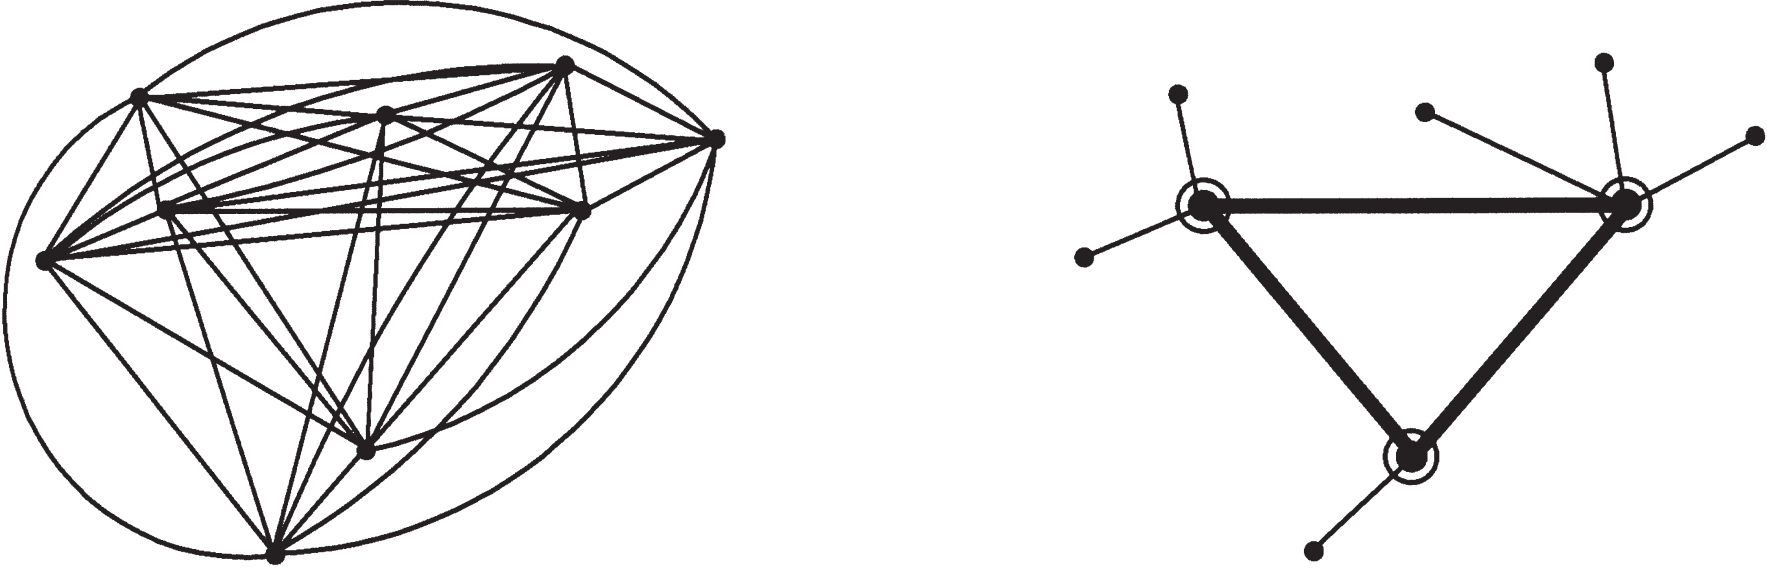
\includegraphics[width=1. \textwidth]{03_figures/Bryan_1999_networks}
    \sourcecenter{\citet{bryan1999hub}}
  \label{fig:different_networks}
\end{figure}

\subsubsection{Spokes vs focus nodes}
\citet{o1987quadratic} presented a hub-and-spoke network as a simple single-assignment model such that non-hub nodes only have one edge, namely the one connecting them to a hub. Thus, a single-hub route network connecting $n$ nodes would only need $n-1$ routes
A hub-and-spoke network








\subsection{Network Theory}
\label{subsec:Network Theory}
We draw on network theory to characterize how airports are connected to each other and analyze what role the individual airport plays in the network of airports. The ultimate aim of this analysis is to assess whether flight prices between airports depend on the role each airport plays in the network. \\
We view airports as nodes in the n

\subsubsection{Network Characteristics}
Given the \textit{spoke and hub} nature of air transport, we expect the network to have some number of airports that are connected to all or most airports in its geographical vicinity, and well connected to similar airports in other regions. This pattern may be repeating to some extent, insofar as there may be regional, national and international hubs, depending on the size of the country. \\ \medskip
In the data, we will expect to see this borne out in the degree distribution, which we (perhaps somewhat stylized) would expect to be bimodal, with a group of airports that have a large degree (hubs), and a larger group of airports with a lower degree (spokes). A more realistic expectation is perhaps, that it is multimodal, with different types of hubs (regional, national, international). It may also be, that these hubs vary so much that actual peaks will be hard to discern in the degree distribution. \\
\medskip
We expect the network to be sparse, i.e. that the number of links is (much) lower than the number of possible links. This reflects the previously described intuition, that small local airports are likely to have a low number of links, particularly relative to the possible number of links. We further expect the network to be connected, in the sense that, given an appropriate time frame, there will always be a path from one airport to the other (through some number of other airports).
% Skriv ovenstående om efter vi har set degree distribution i data.

\subsubsection{A Directed or Undirected Network}
Although individual flights are clearly directed, going from one airport to the other, we will primarily view the network as undirected. The reason being, that connections between airports are typically undirected.
% Tjek at nedenstående er rigtigt i data.
As we will see in the data analysis, flights from airport i to airport j, usually implies flights from airport j to airport i. We believe that this approach to the network of airports is well suited for our analysis, that focusses exclusively on the effect on prices. An analysis of e.g. how delays propagate through the network, would require viewing links as directed and including time in a more intricate manner.\\

\subsubsection{Weighted Network and Temporal Considerations}
For parts of the analysis, we view the network as weighted, i.e. that not all links are considered equal. Specifically, we let the number of flights between airports determine the weight of the link between the airports.
\medskip \\
The considered time frame clearly matters for the characteristics of the network, since not all flights between airports take place every day or even every week. Considering a years worth of flights will produce far more links in the network than considering the flights that take place on a particular day. In practice, we analyse different time periods.

\subsubsection{Air transport as a scale-free network}
A scale-free network is a network whose degree distribution follows a power law, that is: $p_k \sim k^{-\gamma}$. It is a central characteristic of scale-free networks, that they include 'hubs' - nodes that have a far higher degree than the average degree. Air transport is - quite literally - a text-book example of a scale-free network, see chapter 4 of \cite{Barabasi}. As we will see in \ref{sec:empirical}, this is reflected in the degree distribution, where most nodes have a low degree, but some nodes (hubs) have a very high degree.  
% Incorporate insights from Barabasi ch. 4, e.g.  


\subsubsection{Selected Network Measures}
In the course of the analysis, we draw upon a variety of measures to characterize the network. In the choice of measures, we look to \citet{chi2004structural}. In their paper, they use four measures: average degree, clustering coefficient, average shortest path length
\footnote{In their paper, this measure is referred to as diameter, however we follow \citet{Barabasi} and use diameter to denote the maximum distance (node-wise) in the network.}, and efficiency. We further include diameter, %and others?. 
\medskip
\textbf{Average Degree} \\
The degree of node \textit{i} is the number of nodes with which node \textit{i} share an edge. In our cases, the degree of an airport is the number of airports to which it has flights (or that have flights to itself). 
The average degree is then simply the average across nodes. Average degree is calculated as: 
\begin{align}
    \text{Average degree} = \frac{1}{N} \sum_{i = 1}^N k_i = \frac{2L}{N}
\end{align}
\medskip
\textbf{Clustering Coefficient} \\
The clustering coefficient for a given node \textit{i} is given as: 
\begin{align}
    C_i = \frac{2L_i}{k_i(k_i-1)}
    \intertext{The clustering coefficient of the network is then given by:}
    C = \frac{1}{N} \sum^N_{i=1} C_i
\end{align}
The clustering coefficient for a single node is equal to the fraction of possible edges between node \textit{i}'s neighbors (nodes it is connected to) that are found in the network. 
\medskip
\textbf{Average Shortest Path Length} \\
The average shortest path length is defined as: 
\begin{align}
    a = \sum_{s,t \in V} \frac{d(s,t)}{N(N-1)}
\end{align}
Where V is the set of nodes in the network, and N is the number of nodes.

\medskip
\textbf{Diameter} \\
The diameter is the maximum shortest path length between any two nodes in the network. \\
\medskip
\textbf{Betweenness Centrality} \\
Finally, we also calculate the betweenness centrality. For node \textit{i}, this is the fraction of shortest paths between all nodes in the network that pass through node \textit{i}. \cite{brandes2008variants} 
%Notes:



\subsection{Predicting Flight Prices Using Machine Learning Techniques}
In order to predict prices we use a linear prediction model including network characteristics and distance as predictors.\footnote{This section draws on chapter 10 in \citet{raschka2015python}.} We write our prediction model as
$$
p_i = w_0 + W X_i 
$$
where $p_i$ is the price of a given flight, $w_0$ is the bias/intercept, $X_i$ is a vector of predictors, and $W$ is a vector of corresponding weights. 

To find the weights that makes the most accurate predictions we need to define a cost function. The standard cost function estimating a linear model is the \textbf{Mean Squared Error (MSE)}:
$$
\text{MSE}=\frac{1}{N} \sum_i^N (y_i - (w_i + WX_i)^2
$$
We apply some other cost functions such as the LASSO and the RIDGE where complexity is penalized in order to avoid over-fitting.

The cost function is minimized using gradient descent which is a numerical optimization. The model is trained until it has reached threshold or stopped reducing the value of the cost function.%% 

To further reduce the chance of over-fitting, we use a k-fold cross validation. We divide the data into a training set and a test set k times, and estimate and evaluate the model for each set. 

Finally, we tune the hyperparameters in our prediction model using grid search.